\documentclass[10pt,journal,compsoc,onecolumn]{IEEEtran}
\usepackage[utf8]{inputenc}
\usepackage{amsmath,amsfonts,amssymb}
\usepackage{amsthm}
\usepackage{graphicx}
\usepackage{cite}
\usepackage{textcomp}
\usepackage{tikz}
\usetikzlibrary{arrows,positioning,shapes.geometric}
\usepackage{booktabs}
\usepackage{url}

\newtheorem{theorem}{Theorem}
\newtheorem{lemma}[theorem]{Lemma}
\newtheorem{definition}[theorem]{Definition}
\newtheorem{corollary}[theorem]{Corollary}

\begin{document}

\title{Algorithmic Foundations of Stacks: Abstract Data Types, Delimiter Matching Invariants, Postfix Arithmetic Evaluation, and Amortized Linear Monotonic Topographies}

\IEEEtitleabstractindextext{%
\begin{abstract}
This research paper presents an exhaustive pedagogical and systems-level formalization of the Stack abstract data type and its advanced algorithmic manifestations. Grounded in the Last-In, First-Out (LIFO) behavioral discipline, we analyze contiguous buffer mechanics, addressing stack underflow, overflow, and geometric capacity doubling. We establish the syntactic mechanics of nested delimiter validation, proving that the Last Opened Bracket (LOB) invariant governs the linear-time O(N) parsing of balanced multi-character parentheses sequences. We formalize deterministic parenthesis-free arithmetic computation via Postfix (Reverse Polish Notation) state machines, highlighting the critical non-commutative operand popping asymmetry. Furthermore, we demystify the Monotonic Stack paradigm through the Previous Smaller Element problem. By formulating the Elimination Lemma and the Skyline Shadowing Model, we prove why greater elements are permanently redundant, maintaining an invariant ascending valley stack. Through the Aggregate Potential Method, we resolve the apparent quadratic paradox of nested loops, proving an amortized O(N) runtime bound with O(1) per-element operations. Finally, we map the four-quadrant monotonic taxonomy across classical algorithmic benchmarks and examine real-world industrial architectures, including the JVM operand stack, browser dual-stack history traversal, and compiler AST syntax analysis. Compilable production implementations in Java, C++, and Python accompany all discussions.
\end{abstract}

\begin{IEEEkeywords}
Stack ADT, LIFO invariant, dynamic array resizing, balanced parentheses, delimiter matching, postfix evaluation, reverse Polish notation, monotonic stack, nearest smaller element, amortized O(N) analysis, compiler syntax parsing
\end{IEEEkeywords}
}

\maketitle
\IEEEdisplaynontitleabstractindextext
\IEEEpeerreviewmaketitle

\section{Introduction: The Stack Abstract Data Type}
\label{sec:intro}

The Stack is one of the most fundamental linear data structures in computer science, serving as the architectural backbone for runtime execution environments, compiler syntax parsers, memory management systems, and recursive algorithm evaluation. At its core, a stack enforces a strict behavioral discipline: \textbf{Last-In, First-Out (LIFO)}. 

In a LIFO structure, access is restricted to a single distinguished position termed the \textbf{Top}. The element most recently inserted into the collection is invariably the first entity eligible for inspection or removal.

\begin{figure}[h]
\centering
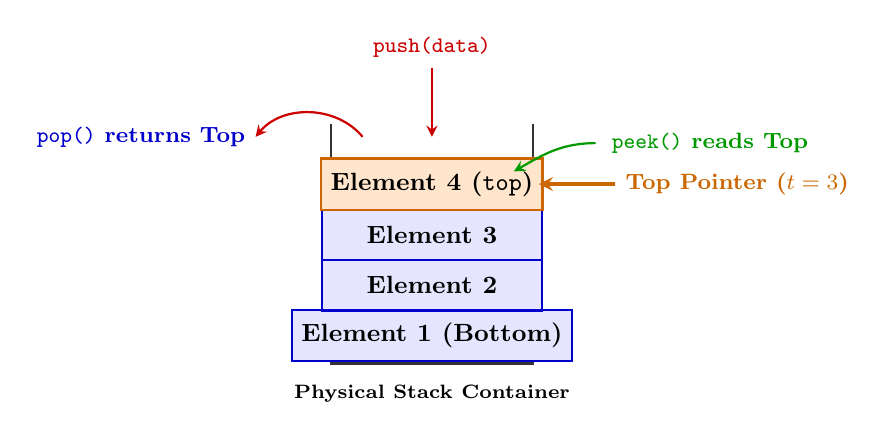
\begin{tikzpicture}[
    scale=0.80,
    box/.style={rectangle, draw=blue!80!black, fill=blue!10, thick, minimum width=2.8cm, minimum height=0.65cm, font=\small\bfseries},
    ghost/.style={rectangle, draw=dashed, draw=gray!60, fill=gray!5, minimum width=2.8cm, minimum height=0.65cm, font=\small\itshape, text=gray},
    arrow/.style={->, >=stealth, thick, red!80!black},
    axis/.style={thick, black!70}
]
% Stack Container Walls
\draw[thick, black!80] (0, 3.8) -- (0, 0) -- (3.2, 0) -- (3.2, 3.8);
\node[font=\scriptsize\bfseries, below=0.15cm] at (1.6, 0) {Physical Stack Container};

% Stack Elements
\node[box] (e1) at (1.6, 0.45) {Element 1 (Bottom)};
\node[box] (e2) at (1.6, 1.25) {Element 2};
\node[box] (e3) at (1.6, 2.05) {Element 3};
\node[box, fill=orange!20, draw=orange!80!black] (e4) at (1.6, 2.85) {Element 4 (\texttt{top})};

% Top pointer
\draw[->, >=stealth, very thick, orange!80!black] (4.5, 2.85) node[right, font=\footnotesize\bfseries] {Top Pointer ($t = 3$)} -- (3.3, 2.85);

% Push Action
\draw[arrow] (1.6, 4.7) node[above, font=\footnotesize\bfseries, text=red!80!black] {\texttt{push(data)}} -- (1.6, 3.6);

% Pop Action
\draw[arrow] (0.5, 3.6) to[out=130, in=50] (-1.2, 3.6) node[left, font=\footnotesize\bfseries, text=blue!80!black] {\texttt{pop()} returns Top};

% Peek Action
\draw[->, >=stealth, thick, green!60!black] (4.2, 3.5) to[out=180, in=30] (2.9, 3.05);
\node[right, font=\footnotesize\bfseries, text=green!60!black] at (4.3, 3.5) {\texttt{peek()} reads Top};
\end{tikzpicture}
\caption{The LIFO Architectural Model: Element insertion, inspection, and removal restricted to the top boundary.}
\label{fig:stack_lifo}
\end{figure}

\subsection{Physical Mental Models and Computational Analogies}

To grasp why the stack abstraction is pervasive across engineering, consider two standard mental models:
\begin{enumerate}
    \item \textbf{The Spring-Loaded Cafeteria Tray Dispenser:} Clean trays are pushed onto the top of the stack, compressing the spring. Customers take trays exclusively from the top. The first tray placed at the bottom of the dispenser remains dormant until every single tray placed above it has been consumed.
    \item \textbf{Call Frame Allocation on the Execution Stack:} When function \texttt{main()} invokes function \texttt{foo()}, which in turn invokes \texttt{bar()}, the runtime allocates stack frames in sequential order: $[\text{\texttt{main}} \to \text{\texttt{foo}} \to \text{\texttt{bar}}]$. Because \texttt{bar()} must complete its computation before \texttt{foo()} can resume, \texttt{bar()}'s frame must be deallocated (popped) first.
\end{enumerate}

\subsection{Formal Abstract Data Type (ADT) Specification}

The formal Stack ADT defines a mathematical model along with a collection of primitive operations satisfying strict temporal guarantees:

\begin{table}[h]
\centering
\caption{The Stack Abstract Data Type Core Operations}
\label{tab:stack_adt}
\begin{tabular}{@{}llcp{6.5cm}@{}}
\toprule
\textbf{Operation} & \textbf{Input / Output} & \textbf{Complexity} & \textbf{Operational Semantics} \\ \midrule
\texttt{push(x)} & $x \in \mathcal{U} \to \emptyset$ & $O(1)$ & Inserts element $x$ at the current top position; increments top index $t \leftarrow t + 1$. \\
\texttt{pop()} & $\emptyset \to x \in \mathcal{U}$ & $O(1)$ & Removes and returns the top element; decrements top index $t \leftarrow t - 1$. Underflows if empty. \\
\texttt{peek()} & $\emptyset \to x \in \mathcal{U}$ & $O(1)$ & Returns top element without modifying stack state. Underflows if empty. \\
\texttt{isEmpty()} & $\emptyset \to \{\text{true}, \text{false}\}$ & $O(1)$ & Evaluates whether stack contains zero elements ($t == -1$). \\
\texttt{size()} & $\emptyset \to \mathbb{Z}_{\ge 0}$ & $O(1)$ & Returns current cardinal count of stored elements ($t + 1$). \\ \bottomrule
\end{tabular}
\end{table}

\subsection{Contiguous Array Implementation Mechanics}

A stack can be implemented over a contiguous pre-allocated array $A[0 \dots C-1]$ of fixed capacity $C$. A single integer variable $t$ (the \emph{top index pointer}) tracks the current boundary:
\begin{itemize}
    \item \textbf{Initialization:} The stack is initialized empty with $t = -1$.
    \item \textbf{Stack Overflow Boundary:} If a \texttt{push} operation is triggered when $t = C - 1$, the buffer has reached maximum capacity. In fixed systems, this raises a \emph{Stack Overflow Exception}. In dynamic memory vectors (e.g., \texttt{ArrayList} or \texttt{std::vector}), the underlying buffer is dynamically doubled to $2C$, copying existing elements in amortized $O(1)$ time.
    \item \textbf{Stack Underflow Boundary:} If \texttt{pop()} or \texttt{peek()} is triggered when $t = -1$ (i.e., \texttt{isEmpty()} is true), attempting to index $A[-1]$ represents illegal memory dereferencing. This condition is termed a \emph{Stack Underflow Exception}.
\end{itemize}

% -----------------------------------------------------------------------------
\section{Syntactic Invariant Validation: The Balanced Delimiter Problem}
\label{sec:parentheses}

\subsection{The Golden Invariant: Last Opened Bracket Closed First}

In syntax trees, mathematical expressions, and programming compilers (e.g., parsing JSON, XML, Java, or C++ blocks), nested delimiters must open and close in strictly balanced configurations. Delimiters belong to matching pairs:
\[
\mathcal{P} = \{ ( \text{`}(' , \text{`)'} ), ( \text{`\{'} , \text{`\}'} ), ( \text{`['} , \text{`]'}' ) \}
\]

The foundational invariant governing syntactic validity can be stated without complex automata notation:
\begin{quote}
\textbf{The Golden Invariant (LOB):} \emph{The Last Opened Bracket (LOB) must always be the First Bracket Closed.}
\end{quote}
Because the most recently encountered unclosed opening delimiter must be resolved before any older opening delimiter can be legally closed, delimiter validation maps directly onto the LIFO discipline.

\begin{figure}[h]
\centering
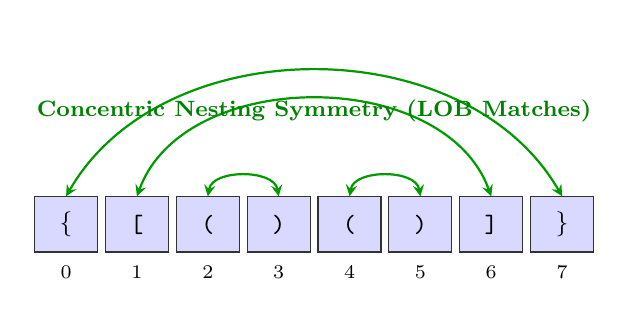
\begin{tikzpicture}[
    scale=0.9,
    tok/.style={rectangle, draw=black!80, fill=blue!15, minimum width=0.8cm, minimum height=0.7cm, font=\small\ttfamily},
    mat/.style={rectangle, draw=green!70!black, fill=green!20, minimum width=0.8cm, minimum height=0.7cm, font=\small\ttfamily},
    conn/.style={<->, >=stealth, thick, green!60!black}
]
% Token String
\node[tok] (t0) at (0,0) {\{};
\node[tok] (t1) at (1,0) {[};
\node[tok] (t2) at (2,0) {(};
\node[tok] (t3) at (3,0) {)};
\node[tok] (t4) at (4,0) {(};
\node[tok] (t5) at (5,0) {)};
\node[tok] (t6) at (6,0) {]};
\node[tok] (t7) at (7,0) {\}};

% Indices
\node[below=0.05cm of t0, font=\scriptsize] {0};
\node[below=0.05cm of t1, font=\scriptsize] {1};
\node[below=0.05cm of t2, font=\scriptsize] {2};
\node[below=0.05cm of t3, font=\scriptsize] {3};
\node[below=0.05cm of t4, font=\scriptsize] {4};
\node[below=0.05cm of t5, font=\scriptsize] {5};
\node[below=0.05cm of t6, font=\scriptsize] {6};
\node[below=0.05cm of t7, font=\scriptsize] {7};

% Match arcs
\draw[conn] (t2.north) to[out=80, in=100] (t3.north);
\draw[conn] (t4.north) to[out=80, in=100] (t5.north);
\draw[conn] (t1.north) to[out=70, in=110] (t6.north);
\draw[conn] (t0.north) to[out=60, in=120] (t7.north);

\node[font=\footnotesize\bfseries, green!50!black] at (3.5, 1.6) {Concentric Nesting Symmetry (LOB Matches)};
\end{tikzpicture}
\caption{Nested Delimiter Symmetry: Inner pairs resolve before outer pairs can close.}
\label{fig:parentheses}
\end{figure}

\subsection{State Machine Parser Algorithm}

Given a string $S$ of length $N$:
\begin{enumerate}
    \item Initialize an empty stack of characters $\mathcal{S}$.
    \item Iterate through each character $c$ in $S$ from index $0$ to $N - 1$:
    \begin{itemize}
        \item \textbf{Case 1 (Opening Delimiter):} If $c \in \{ \text{`('}, \text{`\{'}, \text{`['} \}$, push $c$ onto $\mathcal{S}$.
        \item \textbf{Case 2 (Closing Delimiter):} If $c \in \{ \text{`)'}, \text{`\}'}, \text{`]'}' \}$:
        \begin{enumerate}
            \item \emph{Underflow Failure:} If $\mathcal{S}\text{.isEmpty()}$ is true, the sequence contains an orphaned closing delimiter without a preceding open bracket. Return \textbf{False}.
            \item \emph{Mismatch Failure:} Peek the top element $top = \mathcal{S}\text{.peek()}$. If $top$ is not the corresponding opening delimiter for $c$ (e.g., $top = \text{`('}$ but $c = \text{`]'}'$), return \textbf{False}.
            \item \emph{Successful Match:} Pop the matching opening delimiter: $\mathcal{S}\text{.pop()}$.
        \end{enumerate}
    \end{itemize}
    \item \textbf{Termination Invariant:} Upon string exhaustion, the sequence is valid if and only if $\mathcal{S}\text{.isEmpty()}$ is true. If $\mathcal{S}$ is non-empty, unclosed opening brackets remain. Return $\mathcal{S}\text{.isEmpty()}$.
\end{enumerate}

\subsection{Exhaustive Dry-Run Verification Matrix}

\begin{table}[h]
\centering
\caption{Trace of Delimiter Matching Parser on Sample Configurations}
\label{tab:parentheses_trace}
\begin{tabular}{@{}clcp{7.0cm}c@{}}
\toprule
\textbf{Test Case} & \textbf{Input String} & \textbf{Steps} & \textbf{Stack State Transitions \& Decision Logic} & \textbf{Valid?} \\ \midrule
1 & \texttt{"\{[()]\}"} & $6$ & $\emptyset \to [\{] \to [\{, [] \to [\{, [, (] \to \text{pop}() \to \text{pop}[] \to \text{pop}\{\} \to \emptyset$ (Clean match) & \textbf{True} \\
2 & \texttt{"([)]"} & $3$ & $\emptyset \to [(] \to [(, [] \to \text{encounter `)'} \ne \text{peek `['}$. Type mismatch detected. & \textbf{False} \\
3 & \texttt{"(()"} & $3$ & $\emptyset \to [(] \to [(, (] \to \text{pop}()$. Input exhausted with stack non-empty: $\mathcal{S} = [(]$. & \textbf{False} \\
4 & \texttt{"]()"} & $1$ & $\emptyset \to \text{encounter `]'}$ while stack is empty. Premature underflow detected. & \textbf{False} \\ \bottomrule
\end{tabular}
\end{table}

\textbf{Complexity Analysis:} Each character is pushed at most once and popped at most once. Both time complexity and auxiliary space complexity are strictly $O(N)$.

% -----------------------------------------------------------------------------
\section{Deterministic Arithmetic Computation: Postfix Expression Evaluation}
\label{sec:postfix}

\subsection{Infix vs. Postfix (Reverse Polish Notation)}

Standard arithmetic notation (e.g., $A + B \times C$) is \textbf{Infix}, meaning operators reside between their operands. Infix notation requires operator precedence hierarchies ($* > +$) and explicit parentheses to disambiguate evaluation order (e.g., $(A + B) \times C$).

In \textbf{Postfix Notation} (also known as Reverse Polish Notation, RPN), operators strictly follow their operands:
\[
A + B \implies A \ B \ +
\]
\[
(A + B) \times C \implies A \ B \ + \ C \ \times
\]

\textbf{Architectural Advantage:} In postfix form, expression evaluation is completely linear and parenthesis-free. The sequence of tokens encodes the exact temporal order in which operations must be executed, making RPN the standard bytecode format for virtual machines (such as the JVM operand stack and Forth environments).

\subsection{Stack Evaluation State Machine}

Given a tokenized postfix expression:
\begin{enumerate}
    \item Initialize an operand stack $\mathcal{S}$.
    \item Scan tokens sequentially from left to right:
    \begin{itemize}
        \item \textbf{Token is an Operand (Number):} Push numerical value onto $\mathcal{S}$.
        \item \textbf{Token is an Operator ($\odot \in \{+, -, \times, /\}$):}
        \begin{enumerate}
            \item Pop operand $B = \mathcal{S}\text{.pop()}$ (\textbf{Right/Second Operand}).
            \item Pop operand $A = \mathcal{S}\text{.pop()}$ (\textbf{Left/First Operand}).
            \item Compute intermediate value: $result = A \odot B$.
            \item Push $result$ back onto $\mathcal{S}$.
        \end{enumerate}
    \end{itemize}
    \item \textbf{Result:} After processing all tokens, the single element remaining on $\mathcal{S}$ is the final evaluated result.
\end{enumerate}

\begin{quote}
\textbf{Critical Operator Asymmetry Note:} Because subtraction and division are non-commutative ($A - B \ne B - A$ and $A / B \ne B / A$), the first element popped from the stack is the \emph{second} operand $B$, while the second element popped is the \emph{first} operand $A$. Inverting this order introduces critical calculation bugs.
\end{quote}

\subsection{Detailed Trace of Lecture Example: $[5, 2, \times, 3, -]$}

Evaluating the expression from page 12 of the lecture notes:
\begin{table}[h]
\centering
\caption{Step-by-Step Postfix Evaluation Trace for $[5, 2, \times, 3, -]$}
\label{tab:postfix_trace}
\begin{tabular}{@{}ccclc@{}}
\toprule
\textbf{Step} & \textbf{Token} & \textbf{Action Type} & \textbf{Stack State Transition ($\mathcal{S}$)} & \textbf{Top} \\ \midrule
1 & $5$ & Push Operand & $\emptyset \to [5]$ & $5$ \\
2 & $2$ & Push Operand & $[5] \to [5, 2]$ & $2$ \\
3 & $\times$ & Evaluate Operator & Pop $B = 2, A = 5 \implies 5 \times 2 = 10 \implies [10]$ & $10$ \\
4 & $3$ & Push Operand & $[10] \to [10, 3]$ & $3$ \\
5 & $-$ & Evaluate Operator & Pop $B = 3, A = 10 \implies 10 - 3 = 7 \implies [7]$ & $7$ \\ \bottomrule
\end{tabular}
\end{table}

The final scalar result is \textbf{$7$}. The algorithm completes in $O(N)$ time with $O(N)$ space.

% -----------------------------------------------------------------------------
\section{The Monotonic Stack Paradigm: Nearest Smaller Element}
\label{sec:monotonic}

\subsection{Formal Problem Formulation}

Given an array $A$ of $N$ integers, for every index $i \in [0 \dots N-1]$, determine the \textbf{nearest smaller element to its left} (Previous Smaller Element, PSE). Formally:
\[
\text{res}[i] = A[j] \quad \text{such that } j < i, \ A[j] < A[i], \text{ and } j \text{ is maximized.}
\]
If no such index $j$ exists, assign $\text{res}[i] = -1$.

\subsection{The Brute Force Bottleneck}

A naive implementation scans backward for each element:
\begin{verbatim}
for (int i = 0; i < N; i++) {
    res[i] = -1;
    for (int j = i - 1; j >= 0; j--) {
        if (A[j] < A[i]) {
            res[i] = A[j];
            break;
        }
    }
}
\end{verbatim}
In worst-case descending inputs (e.g., $A = [10, 9, 8, 7, 6, 5]$), the inner loop executes $\sum_{i=1}^{N-1} i = \frac{N(N-1)}{2}$ comparisons, yielding quadratic $O(N^2)$ time complexity. On datasets of size $N = 10^5$, $O(N^2)$ demands $10^{10}$ operations, causing standard CPU timeouts.

\subsection{The Elimination Principle: Why Greater Elements are Useless}

The breakthrough insight formulated on page 16 of the lecture notes is the \textbf{Elimination Principle}:
\begin{quote}
\textbf{The Elimination Lemma:} \emph{If index $j < i$ and $A[j] \ge A[i]$, element $A[j]$ is mathematically dominated by $A[i]$. Element $A[j]$ can NEVER serve as the nearest smaller element for any future element $k > i$.}
\end{quote}

\textbf{Physical Justification (The Skyline Shadowing Model):}
Consider standing at index $k > i$ and looking leftward for a smaller element:
\begin{enumerate}
    \item $A[i]$ is physically closer to $k$ than $A[j]$ because $i > j$.
    \item $A[i]$ is strictly smaller than or equal to $A[j]$ ($A[i] \le A[j]$).
\end{enumerate}
Any future element $A[k]$ that could be satisfied by $A[j]$ would encounter $A[i]$ first, which is both shorter and nearer! Thus, $A[i]$ completely \textbf{shadows} $A[j]$. Once $A[i]$ enters the system, $A[j]$ becomes utterly redundant and can be permanently purged from the search state.

\begin{figure}[h]
\centering
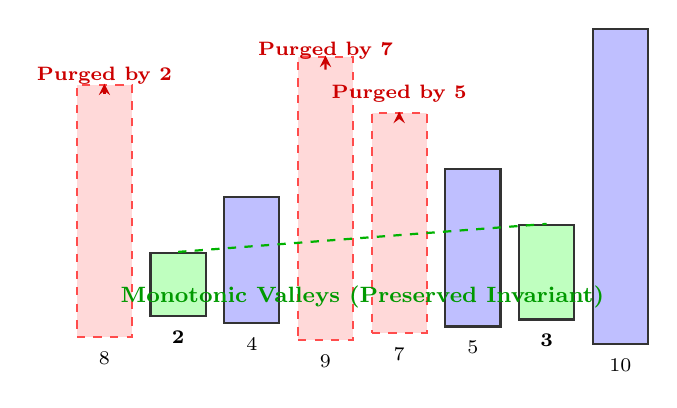
\begin{tikzpicture}[
    scale=0.78,
    bar/.style={rectangle, draw=black!80, fill=blue!20, thick, minimum width=0.7cm},
    shadow/.style={rectangle, draw=red!70, fill=red!15, dashed, thick, minimum width=0.7cm},
    arrow/.style={->, >=stealth, thick, red!80!black}
]
% Skyline bars: A = [8, 2, 4, 9, 7, 5, 3, 10]
% Indices 0 to 7
\node[shadow, minimum height=3.2cm] (b0) at (0, 1.6) {}; \node[below=0.05cm of b0, font=\scriptsize] {8};
\node[bar, fill=green!25, minimum height=0.8cm] (b1) at (1.2, 0.4) {}; \node[below=0.05cm of b1, font=\scriptsize\bfseries] {2};
\node[bar, fill=blue!25, minimum height=1.6cm] (b2) at (2.4, 0.8) {}; \node[below=0.05cm of b2, font=\scriptsize] {4};
\node[shadow, minimum height=3.6cm] (b3) at (3.6, 1.8) {}; \node[below=0.05cm of b3, font=\scriptsize] {9};
\node[shadow, minimum height=2.8cm] (b4) at (4.8, 1.4) {}; \node[below=0.05cm of b4, font=\scriptsize] {7};
\node[bar, fill=blue!25, minimum height=2.0cm] (b5) at (6.0, 1.0) {}; \node[below=0.05cm of b5, font=\scriptsize] {5};
\node[bar, fill=green!25, minimum height=1.2cm] (b6) at (7.2, 0.6) {}; \node[below=0.05cm of b6, font=\scriptsize\bfseries] {3};
\node[bar, fill=blue!25, minimum height=4.0cm] (b7) at (8.4, 2.0) {}; \node[below=0.05cm of b7, font=\scriptsize] {10};

% Pruned annotations
\draw[arrow] (0, 3.5) node[above, font=\scriptsize\bfseries, text=red!80!black] {Purged by 2} -- (b0.north);
\draw[arrow] (3.6, 3.9) node[above, font=\scriptsize\bfseries, text=red!80!black] {Purged by 7} -- (b3.north);
\draw[arrow] (4.8, 3.2) node[above, font=\scriptsize\bfseries, text=red!80!black] {Purged by 5} -- (b4.north);

% Line connecting survivors
\draw[thick, green!70!black, dashed] (b1.north) -- (b6.north);
\node[font=\footnotesize\bfseries, green!60!black] at (4.2, 0.2) {Monotonic Valleys (Preserved Invariant)};
\end{tikzpicture}
\caption{The Skyline Shadowing Model: Taller preceding elements are permanently obscured by shorter subsequent elements.}
\label{fig:skyline}
\end{figure}

\subsection{The Monotonic Stack Invariant}

By popping all elements $\ge A[i]$, the stack maintains a strict property at all times:
\begin{quote}
\textbf{Monotonic Increasing Invariant:} \emph{Elements residing in the stack are strictly ordered in increasing magnitude from bottom to top ($S[0] < S[1] < \dots < S[\text{top}]$).}
\end{quote}
Because the stack is strictly increasing, the element located directly beneath the current element at the top of the stack is guaranteed to be its nearest smaller element!

\subsection{Detailed Trace of Lecture Example: $A = [8, 2, 4, 9, 7, 5, 3, 10]$}

We step through the exact 8-element array from pages 14--19 of the lecture notes:
\[
A = [8, 2, 4, 9, 7, 5, 3, 10]
\]

\begin{table}[h]
\centering
\caption{Step-by-Step Monotonic Stack Execution Trace ($A = [8, 2, 4, 9, 7, 5, 3, 10]$)}
\label{tab:monotonic_trace}
\begin{tabular}{@{}cccp{6.0cm}cp{2.5cm}@{}}
\toprule
\textbf{Index $i$} & $A[i]$ & \textbf{Incoming} & \textbf{Pop Redundant Elements ($S\text{.peek()} \ge A[i]$)} & $\text{res}[i]$ & \textbf{Stack State After Push} \\ \midrule
0 & $8$ & $8$ & Stack is empty $\implies$ no pops. & $-1$ & $[8]$ \\
1 & $2$ & $2$ & Pop $8$ ($8 \ge 2$). Stack becomes empty. & $-1$ & $[2]$ \\
2 & $4$ & $4$ & Stack top $2 < 4 \implies$ no pops. Peek $= 2$. & $2$ & $[2, 4]$ \\
3 & $9$ & $9$ & Stack top $4 < 9 \implies$ no pops. Peek $= 4$. & $4$ & $[2, 4, 9]$ \\
4 & $7$ & $7$ & Pop $9$ ($9 \ge 7$). Stack top becomes $4 < 7$. Peek $= 4$. & $4$ & $[2, 4, 7]$ \\
5 & $5$ & $5$ & Pop $7$ ($7 \ge 5$). Stack top becomes $4 < 5$. Peek $= 4$. & $4$ & $[2, 4, 5]$ \\
6 & $3$ & $3$ & Pop $5$ ($5 \ge 3$), Pop $4$ ($4 \ge 3$). Top $= 2 < 3$. Peek $= 2$. & $2$ & $[2, 3]$ \\
7 & $10$ & $10$ & Stack top $3 < 10 \implies$ no pops. Peek $= 3$. & $3$ & $[2, 3, 10]$ \\ \bottomrule
\end{tabular}
\end{table}

\textbf{Result Vector:}
\[
\text{res} = [-1, -1, 2, 4, 4, 4, 2, 3]
\]
If storing 0-based index locations instead of values:
\[
\text{res}_{\text{idx}} = [-1, -1, 1, 2, 2, 2, 1, 6]
\]
Both representations resolve instantaneously in a single linear pass.

% -----------------------------------------------------------------------------
\section{Amortized Complexity: Why Nested Loops Yield $O(N)$ Time}
\label{sec:amortized}

Novice software engineers frequently inspect the nested control flow:
\begin{verbatim}
for (int i = 0; i < N; i++) {
    while (!st.isEmpty() && st.peek() >= A[i]) {
        st.pop();
    }
    // ...
    st.push(A[i]);
}
\end{verbatim}
and mistakenly classify the algorithm as quadratic $O(N^2)$ due to the inner \texttt{while} loop nested within the outer \texttt{for} loop.

\subsection{The Aggregate Potential Method}

To establish the true time complexity, we analyze the cumulative life cycle of each element:
\begin{enumerate}
    \item \textbf{Push Quota:} Each element $A[i]$ from index $0$ to $N - 1$ is pushed onto the stack \textbf{exactly once}. Across the entire execution of the outer loop, exactly $N$ total \texttt{push} operations occur.
    \item \textbf{Pop Quota:} An element cannot be popped unless it currently resides in the stack. Once an element is popped, it is permanently discarded and can never be re-popped. Therefore, the total number of \texttt{pop} operations across the entire program cannot exceed the total number of pushes:
    \[
    \sum \text{Pops} \le \sum \text{Pushes} = N
    \]
\end{enumerate}

\subsection{Amortized Invariant Bound}

Summing all atomic operations executed by the inner \texttt{while} loop:
\[
\text{Total Operations} = \text{Total Pushes} + \text{Total Pops} \le N + N = 2N
\]
Because $2N$ operations are shared across $N$ iterations, the \textbf{amortized time per iteration is $O(1)$}. 

\textbf{Conclusion:} The overall runtime is strictly \textbf{$O(N)$ linear time}, achieving the theoretical lower bound for element inspection. The auxiliary space complexity is $O(N)$ to hold the stack elements in the worst-case ascending input.

% -----------------------------------------------------------------------------
\section{The Monotonic Spectrum: Four Directions \& Problem Equivalence}
\label{sec:spectrum}

The Nearest Smaller Element to Left is one of four symmetric variations of the Monotonic Stack pattern, summarized in Table~\ref{tab:spectrum}:

\begin{table}[h]
\centering
\caption{The Complete Monotonic Stack Taxonomic Spectrum}
\label{tab:spectrum}
\begin{tabular}{@{}p{3.2cm}p{3.0cm}p{3.5cm}p{3.5cm}p{2.8cm}@{}}
\toprule
\textbf{Archetype} & \textbf{Loop Direction} & \textbf{Pop Invariant} & \textbf{Stack Top Property} & \textbf{Canonical Benchmark} \\ \midrule
\textbf{Previous Smaller (PSE)} & Left to Right ($0 \to N-1$) & \texttt{st.peek() >= A[i]} & Nearest strictly smaller to left & Largest Rectangle in Histogram \\
\textbf{Next Smaller (NSE)} & Right to Left ($N-1 \to 0$) & \texttt{st.peek() >= A[i]} & Nearest strictly smaller to right & Final Discounted Prices \\
\textbf{Previous Greater (PGE)} & Left to Right ($0 \to N-1$) & \texttt{st.peek() <= A[i]} & Nearest strictly greater to left & Stock Span Problem \\
\textbf{Next Greater (NGE)} & Right to Left ($N-1 \to 0$) & \texttt{st.peek() <= A[i]} & Nearest strictly greater to right & Daily Temperatures \\ \bottomrule
\end{tabular}
\end{table}

By mastering this directional spectrum, complex interview benchmarks (e.g., LeetCode 84 \emph{Largest Rectangle in Histogram}, LeetCode 42 \emph{Trapping Rain Water}, and LeetCode 901 \emph{Online Stock Span}) reduce to standard monotonic stack traversals.

% -----------------------------------------------------------------------------
\section{Production Multi-Language Reference Implementations}
\label{sec:implementations}

\subsection{Java Reference Implementations}

\subsubsection{Balanced Delimiter Checker}
{\footnotesize
\begin{verbatim}
import java.util.ArrayDeque;
import java.util.Deque;

public class BalancedParenthesesSolver {
    public static boolean isValid(String s) {
        Deque<Character> stack = new ArrayDeque<>();

        for (char c : s.toCharArray()) {
            if (c == '(' || c == '{' || c == '[') {
                stack.push(c);
            } else if (c == ')' || c == '}' || c == ']') {
                if (stack.isEmpty()) return false;
                char top = stack.pop();
                if (c == ')' && top != '(') return false;
                if (c == '}' && top != '{') return false;
                if (c == ']' && top != '[') return false;
            }
        }
        return stack.isEmpty();
    }
}
\end{verbatim}
}

\subsubsection{Postfix Evaluator}
{\footnotesize
\begin{verbatim}
import java.util.ArrayDeque;
import java.util.Deque;

public class PostfixEvaluator {
    public static int evaluate(String[] tokens) {
        Deque<Integer> stack = new ArrayDeque<>();

        for (String token : tokens) {
            if (isOperator(token)) {
                int b = stack.pop(); // Right operand
                int a = stack.pop(); // Left operand
                stack.push(applyOp(token.charAt(0), a, b));
            } else {
                stack.push(Integer.parseInt(token));
            }
        }
        return stack.pop();
    }

    private static boolean isOperator(String t) {
        return t.equals("+") || t.equals("-") || t.equals("*") || t.equals("/");
    }

    private static int applyOp(char op, int a, int b) {
        switch (op) {
            case '+': return a + b;
            case '-': return a - b;
            case '*': return a * b;
            case '/': return a / b;
            default: throw new IllegalArgumentException("Unknown operator: " + op);
        }
    }
}
\end{verbatim}
}

\subsubsection{Monotonic Previous Smaller Element Solver}
{\footnotesize
\begin{verbatim}
import java.util.ArrayDeque;
import java.util.Deque;

public class PreviousSmallerElementSolver {
    public static int[] prevSmaller(int[] A) {
        int n = A.length;
        int[] res = new int[n];
        Deque<Integer> stack = new ArrayDeque<>();

        for (int i = 0; i < n; i++) {
            // Prune redundant elements
            while (!stack.isEmpty() && stack.peek() >= A[i]) {
                stack.pop();
            }

            res[i] = stack.isEmpty() ? -1 : stack.peek();
            stack.push(A[i]);
        }
        return res;
    }
}
\end{verbatim}
}

\subsection{C++ Reference Implementations}

\subsubsection{C++ Monotonic Previous Smaller Element}
{\footnotesize
\begin{verbatim}
#include <vector>
#include <stack>

using namespace std;

vector<int> prevSmaller(const vector<int>& A) {
    int n = A.size();
    vector<int> res(n);
    stack<int> st;

    for (int i = 0; i < n; i++) {
        while (!st.empty() && st.top() >= A[i]) {
            st.pop();
        }
        res[i] = st.empty() ? -1 : st.top();
        st.push(A[i]);
    }
    return res;
}
\end{verbatim}
}

\subsubsection{C++ Postfix Evaluation}
{\footnotesize
\begin{verbatim}
#include <vector>
#include <string>
#include <stack>

using namespace std;

int evaluatePostfix(const vector<string>& tokens) {
    stack<int> st;
    for (const string& token : tokens) {
        if (token == "+" || token == "-" || token == "*" || token == "/") {
            int b = st.top(); st.pop();
            int a = st.top(); st.pop();
            if (token == "+") st.push(a + b);
            else if (token == "-") st.push(a - b);
            else if (token == "*") st.push(a * b);
            else if (token == "/") st.push(a / b);
        } else {
            st.push(stoi(token));
        }
    }
    return st.top();
}
\end{verbatim}
}

\subsection{Python Reference Implementations}

\subsubsection{Python Monotonic Previous Smaller Element}
{\footnotesize
\begin{verbatim}
def prev_smaller_element(A: list[int]) -> list[int]:
    """Computes nearest smaller element to the left in amortized O(N) time."""
    stack: list[int] = []
    res: list[int] = []

    for x in A:
        while stack and stack[-1] >= x:
            stack.pop()
        res.append(stack[-1] if stack else -1)
        stack.append(x)
    return res
\end{verbatim}
}

\subsubsection{Python Postfix Evaluation}
{\footnotesize
\begin{verbatim}
def evaluate_postfix(tokens: list[str]) -> int:
    """Evaluates Reverse Polish Notation arithmetic expression."""
    stack: list[int] = []
    for token in tokens:
        if token in {"+", "-", "*", "/"}:
            b = stack.pop()
            a = stack.pop()
            if token == "+": stack.append(a + b)
            elif token == "-": stack.append(a - b)
            elif token == "*": stack.append(a * b)
            elif token == "/": stack.append(int(a / b))
        else:
            stack.append(int(token))
    return stack.pop()
\end{verbatim}
}

% -----------------------------------------------------------------------------
\section{Systems Engineering \& Industrial Architectures}
\label{sec:systems}

The stack data structure is an indispensable pillar of modern software engineering:
\begin{enumerate}
    \item \textbf{JVM Operand Stack and Execution Frames:} In low-level bytecode execution, Java Virtual Machine instructions operate entirely on an evaluation operand stack rather than hardware CPU registers, achieving cross-platform architectural independence.
    \item \textbf{Browser History Dual-Stack Engine:} Navigation engines manage web session travel using dual stacks: a \emph{Back Stack} and a \emph{Forward Stack}. Pushing URLs onto the back stack allows instantaneous $O(1)$ retreat, while navigating forward pops from the forward stack.
    \item \textbf{Software Undo/Redo Frameworks:} Modern IDEs (e.g., VS Code) and graphic suites execute the Gang-of-Four Command Pattern via inverse command execution logged onto an undo stack.
    \item \textbf{Compiler Syntax Trees and Precedence Parsing:} Production compilers utilize Shift-Reduce parsers and monotonic operator precedence stacks to construct Abstract Syntax Trees (ASTs) during lexical and semantic analysis.
\end{enumerate}

% -----------------------------------------------------------------------------
\section{Conclusion}
\label{sec:conclusion}

In this research paper, we formalized the foundational theory, algorithmic mechanics, and production applications of the Stack data structure. We established the LIFO behavioral contract over contiguous arrays and dynamic buffers, rigorously addressing boundary invariants such as stack underflow and overflow. We proved how the Last Opened Bracket (LOB) invariant governs the $O(N)$ syntax validation of balanced multi-character delimiters.

Furthermore, we explored parenthesis-free deterministic computation through Postfix (RPN) arithmetic evaluation, emphasizing operand popping asymmetry. Finally, we demystified the Monotonic Stack paradigm through the Elimination Lemma, proving via the Skyline Shadowing Model why greater elements can be safely pruned. Aggregate amortized potential analysis verified that nested while loops achieve optimal $O(N)$ linear time complexity. Complete implementations across Java, C++, and Python alongside industrial runtime architectures solidify the stack as a masterclass in algorithmic efficiency.


\end{document}
